En este capítulo se explica como se utiliza el ecosistema, con intención de que se pueda entender el propósito de cada extensión. En los capítulos siguientes se entrará en más detalle con respecto a la toma de decisiones en el diseño y como se ha logrado implementar todo el ecosistema 

\section{El Núcleo de {\tt gh edu}: Core}

El diseño de la extensión \verb|gh-edu| sigue el \gls{strategy pattern} y consta de un código núcleo (\verb|core|) que coordina las estrategias y extensiones. Algunas de las estrategias más básicas forman parte del código núcleo que se provee con la \verb|gh-extension| \verb|gh-edu|.

Todos los comandos de \verb|gh-edu|  se pueden ejecutar desde la línea de comandos y cuando es apropiado cuentan con un modo interactivo. La figura \ref{fig:ghEduHelp} muestra los subcomandos disponibles en el núcleo.

\begin{figure}[h]
    \centering
    \makebox[\textwidth][c]{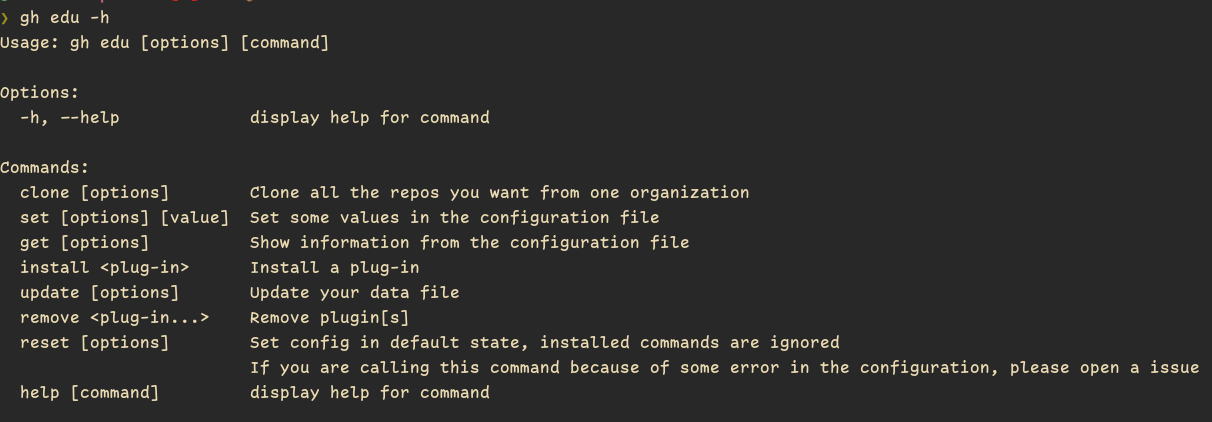
\includegraphics[width=\textwidth]{images/gh-edu-help.png}}
    \caption{Ayuda general de gh edu}
    \label{fig:ghEduHelp}
\end{figure}

Para este apartado es relevante saber que \verb|gh-edu| trabaja en torno a un archivo de datos o registro llamado \verb|data.json|.

Este archivo de datos guarda información
\begin{itemize}
    \item de las extensiones instaladas 
    \item de la versión y configuración de las extensiones instaladas,
    \item de información proveida por las extensiones a solicitud del usuario
    \item del usuario y de la configuración del usuario 
    \item del estado actual del sistema \verb|gh-edu| (por ejemplo, cuál es la organización GitHub por defecto)
    \item de datos obtenidos desde la API de GitHub y que han sido cacheados
\end{itemize}
 este fichero se guarda de forma persistente en \verb|$HOME/.config/gh-edu/data.json|. Este directorio esta siempre bajo control de versiones y puede estar enlazado a un remoto llamado \verb|https://github.com/github-user:/gh-edu-profile|.

Dicho fichero es único y privado para cada usuario y se obtiene de una de estas dos formas:
\begin{itemize}
    \item Se crea uno nuevo a partir de una plantilla base, la cual tiene los elementos mínimos para dar el fichero por válido, o 
    \item Se descarga automáticamente si el usuario tiene uno propio dentro de un repositorio en GitHub en su cuenta con el nombre \verb|<github-user>/gh-edu-profile|. 
\end{itemize}

Se entrará más en detalle sobre \verb|data.json| en el capítulo \textbf{Diseño} \ref{diseño:data}.

\subsection{Subcomando set}
Comando importante, utilizado para establecer la configuración en el fichero de datos
\begin{figure}[h]
    \centering
    \makebox[\textwidth][c]{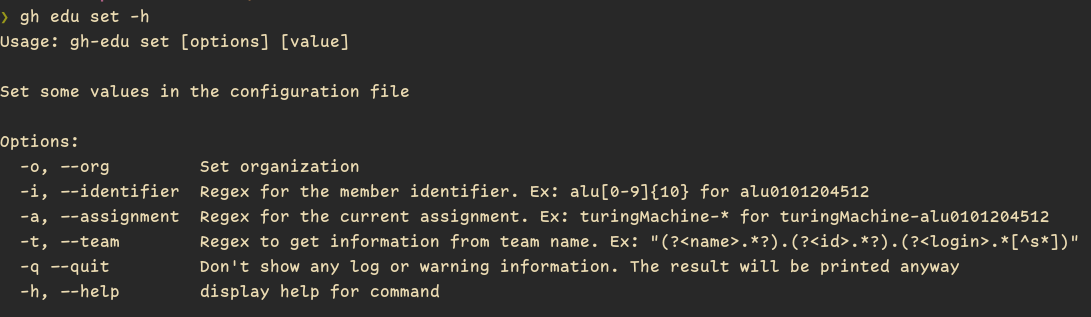
\includegraphics[width=\textwidth]{images/set-help.png}}
    \caption{Ayuda de gh edu set}
    \label{fig:ghEduSetHelp}
\end{figure}

\begin{itemize}
    \item \textbf{-o, -{}-org.} Específica la organización con la que estamos trabajando actualmente. En la mayoría de universidades, las organizaciones de GitHub suelen estar asociados a las asignaturas.
    Ejemplo de uso: \verb|gh edu set -o gh-cli-for-education|, si pertenecemos a la organización se registrará como organización actual y se guardará como cache a los miembros pertenecientes de la organización.
    Si no se le pasa un valor, se activará \verb|fzf| para poder elegir entre las organizaciones a las que el usuario pertenezca.
    \item \textbf{-q, -{}-quiet.} No se muestra ninguna información por pantalla, más allá del resultado y los errores.
    \item \textbf{-i, -{}-identifier.} Expresión regular para identificar los identificadores de los alumnos, en el caso de la ULL utilizamos \verb|alu| seguido de 10 números del 0 al 9. que se corresponde con la expresión regular \verb|alu[0-9]\{10\}|
    \item \textbf{-t, -{}-team.} Expresión regular para poder extraer información del nombre de los equipos. Está pensada para que se utilice con agrupamientos con nombre (``named captured group``). Por ejemplo, la expresión regular:\\ \verb|(?<name>.*?).(?<id>.*?).(?<login>.*[^s*])|\\
    Aplicada sobre el siguiente nombre de equipo:\\
    \verb|cristo-garcia-gonzález.alu0101204512.ggcristo|\\
    Es capaz de generar automáticamente la siguiente información:
    \begin{itemize}
        \item \textbf{name:} cristo-garcia-gonzález
        \item \textbf{id:} alu0101204512
        \item \textbf{login:} ggcristo
    \end{itemize}
    \item \textbf{-a, -{}-assignment}. Expresión regular para marcar los repositorios sobre los que se quiere trabajar. Normalmente, se le asigna un repositorio a cada alumno por asignación/tarea. Por ejemplo: \verb|turingMachine-.*| en el caso de que los repositorios empiecen por \verb|turingMachine| como podría ser \verb|turingMachine-alu0101204512|.
\end{itemize}
El uso que se les dé a estos campos depende deliberadamente de cada desarrollador y profesor.

\subsection{El subcomando core {\tt get}}
\begin{figure}
    \centering
    \makebox[\textwidth][c]{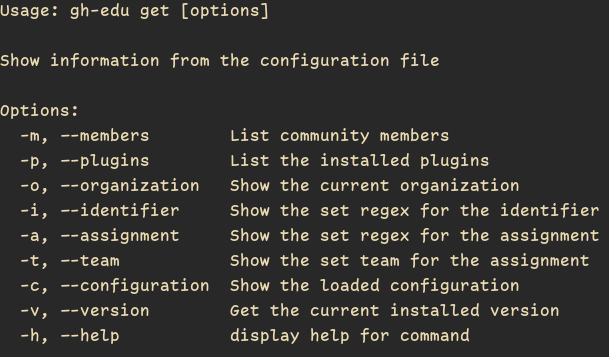
\includegraphics[width=\textwidth]{images/get-help.png}}
    \caption{Ayuda de gh edu get}
    \label{fig:ghEduGetHelp}
\end{figure}
El comando \verb|get| muestra la información que se tiene actualmente
\begin{itemize}
    \item \textbf{-m, -{}-members.} Muestra los miembros de la organización establecida. Lee de la caché, si es posible.
    \item \textbf{-p, -{}-plugins.} Lista las extensiones y comandos disponibles tanto los que vienen con el core (builtin) como los instalados por el usuario.
    \item \textbf{-o, -{}-org.} Muestra la organización marcada.
    \item \textbf{-i, -{}-identifier}. Muestra la expresión regular establecida para detectar los identificadore de los alumnos.
    \item \textbf{-a, -{}-assignment.} Muestra la expresión regular establecida para filtrar los repositorios deseados.
    \item \textbf{-t, -{}-team.} Muestra la expresión regular establecida para recolectar información de los nombres de los equipos.
    \item \textbf{-v, -{}-version.} Muestra la versión instalada.
    \item \textbf{-c, -{}-configuration.} Muestra por pantalla la toda la configuración y datos cargados.
\end{itemize}

\subsection{El subcomando core {\tt clone}}
El comando \verb|clone| solo tiene dos opciones \verb|--org| por si queremos clonar de una organización en concreto sin tener que cambiar la organización establecida y \verb|--quiet| para solo mostrar los mensajes de errores (y \verb|--help|).
Este comando fue planeado para clonar varios repositorios en paralelo usando la librería \href{https://www.npmjs.com/package/concurrently}{concurrently}

\begin{figure}[H]
    \centering
    \makebox[\textwidth][c]{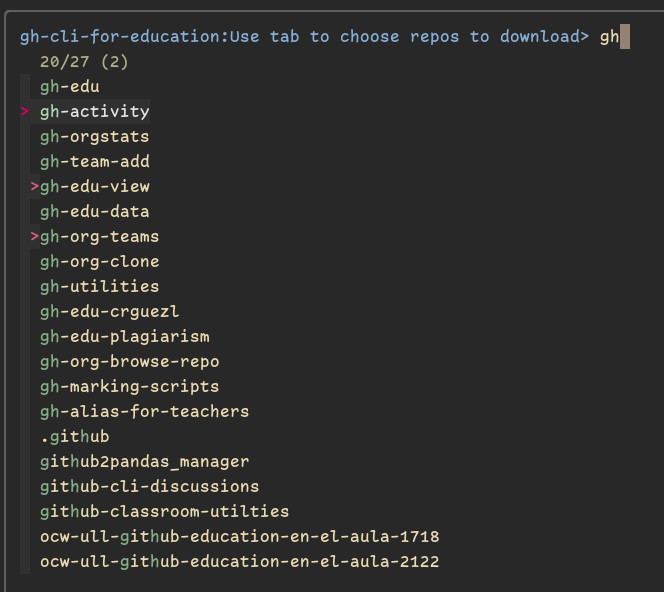
\includegraphics[width=\textwidth]{images/clone.png}}
    \caption{clone usando fzf}
    \label{fig:clone}
\end{figure}

En la figura \ref{fig:clone} se ve la interfaz de \verb|clone| con \verb|fzf|, arriba a la izquierda aparece el nombre de la organización y podemos seleccionar múltiples repositorios presionando \emph{TAB} y filtrarlos de forma difusa (nótese como \verb|.github|, el cual no es una coincidencia exacta, aparece en la lista), para aceptar se pulsa \emph{ENTER}.

\subsection{El subcomando {\tt install}}
Como su nombre indica \verb|install| instala extensiones añadiendo más comandos al sistema. No acepta otro argumento más que el nombre de la extensión que queremos instalar y solamente tiene el \verb|flag| \verb|--quiet|, con la misma funcionalidad que el resto de extensiones.

El código de las extensiones tiene que estar alojado en GitHub y solo funciona con la rama por defecto.

El comando se ejecuta de la siguiente forma:\\
\verb|gh edu install <organización/nombre_extension>|

Ejemplo:

\begin{verbatim}
        gh edu install crguezl/gh-edu-browse
        Installing crguezl/gh-edu-browse ...
        Plugin installed in system
        Setting up configuration...
        crguezl/gh-edu-browse installed as browse
\end{verbatim}
Pero si la extensión es \emph{first-party}, es decir, pertenece a la organización \verb|gh-cli-for-education|, no es necesario especificar la organización. Por ende:\\
\verb|gh edu install gh-cli-for-education/view|, es equivalente a \verb|gh edu install view|

\subsection{El subcomando {\tt remove}}
Elimina las extensiones instaladas por el comando \verb|install|. No puede eliminar los comandos \emph{bultin}.\\
El comando se ejecuta de la siguiente forma:\\
\verb|gh edu remove <nombre_extension1> <nombre_extension2> ... <nombre_extensionN>|

\subsection{El subcomando {\tt update}}

\begin{figure}[htb]
    \centering
    \makebox[\textwidth][c]{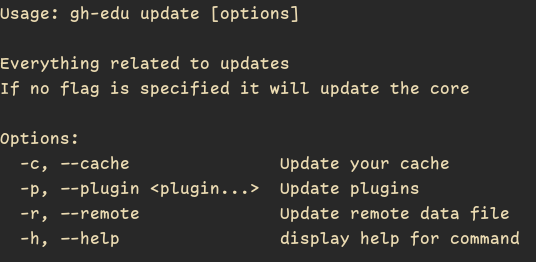
\includegraphics[width=\textwidth]{images/updateHelp.png}}
    \caption{Ayuda de get update}
    \label{fig:updateHelp}
\end{figure}

El subcomando \verb|update| se encarga de todo lo relacionado con las actualizaciones.
\begin{itemize}
    \item \textbf{-c, -{}-cache.} Actualiza todos los valores posibles de la caché. No es un comando esencial, especialmente cuando algunos comandos ya actualizan ciertas partes de la caché, pero es recomendable correrlo desde que se obtenga el fichero de datos data.json.
    \item \textbf{-p, -{}-plugin.} Actualiza una o varías extensiones. Si no tiene un argumento, actualiza todas las extensiones instaladas.
    \item \textbf{-r -{}-remote.} Actualiza el repositorio gh-edu-profile con los datos locales. En caso de no existir se le pregunta al usuario si quiere crear dicho repositorio.
    \item \textbf{Sin argumentos ni \emph{flags}.} Si el usuario ejecuta el comando sin argumentos, el propio \verb|core| se actualizará. Es equivalente a \verb|gh extension upgrade gh-edu|. Fue creado para mantener la simetría con el resto de comandos.
\end{itemize}

\subsection{El subcomando {\tt reset}}
Restaura la configuración a su estado original dejando intacto la información sobre los comandos instalados, si también se desea borrar dicha información se puede usar el flag \verb|--force|, aunque no es recomendable, ya que generaría una incongruencia con las extensiones que están realmente instaladas en el sistema y la propia información del sistema.

Este comando existe por meros motivos de depuración y en caso de que un error en la implementación del sistema lleve al usuario a un estado anormal. No se debe de usar con regularidad.

\section{La Extensión {\tt view}}
Es una pequeña extensión para mostrar información relevante sobre la organización, por lo que es necesario tener una organización establecida.

Dentro del contexto del TFG se ha desarrollado un único comando \verb|members| que muestra información sobre los miembros de la organización. Se espera ampliarlo para que también muestre otro tipo de información que pueda ser relevante al profesorado y alumnado (vease \ref{conclusion}).

Esta extensión también aprovecha la expresión regular del identificador guardado en data.json para intentar conseguir los identificadores de los alumnos leyendo varios campos en su cuenta de GitHub

Se puede ejecutar directamente como: \verb|gh edu view members| o añadir el flag \verb|--id| para usar un identificador que tendrá prioridad sobre el establecido en \verb|data|.
\begin{figure}[H]
    \centering
    \makebox[\textwidth][c]{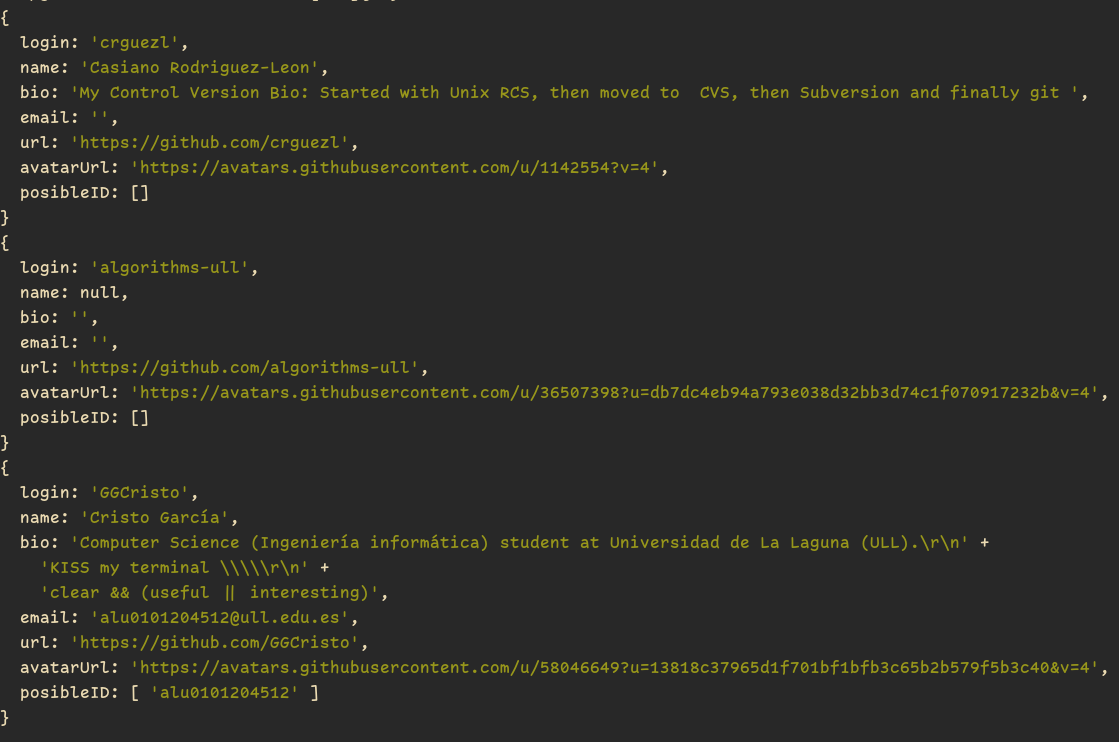
\includegraphics[width=\textwidth]{images/view.png}}
    \caption{Ejemplo de uso de gh view con --id ``alu[0-9]\{10\}``}
    \label{fig:view}
\end{figure}

\section{La Extensión {\tt data}}

Ha sido creado para manejar y guardar información variada de los alumnos.

Para instalarla:
\begin{verbatim}
    gh edu install data
\end{verbatim}

Tiene tres comandos principales: \verb|log|, \verb|teams| y \verb|team-add|:


\begin{verbatim}
    $ gh edu data -h
    Usage: gh-edu-data [options] [command]
    
    Options:
      -h, --help                 display help for command
    
    Commands:
      log [options] <inputFile>  Get relevant information about you students
      teams [options]            Get relevant information about you students using
                                 teams
      team-add [options]         Create teams with certain patterns to get
                                 information later on. Empty spaces will become '-'
      help [command]             display help for command
\end{verbatim}

\subsection{El subcomando {\tt log}}
El objetivo de \verb|log| es principalmente relacionar la cuenta institucional de un alumno con su cuenta de GitHub y conseguir información extra que le pueda ser de utilidad al profesor.

\begin{verbatim}
    gh edu data log -h
    Usage: gh-edu-data log [options] <inputFile>
    
    Get relevant information about you students
    
    Options:
      -o, --output <outputFile>  File to write the resulting data. If not specified
                                 it will write the result to the standard output
      -c, --cache                Cache the information in the configuration file
      -q, --quiet                Don't show any output, except errors
      -h, --help                 display help for command
\end{verbatim}
Se necesita de un fichero inicial con información que el profesor tenga de los alumnos. Dicho fichero de entrada tiene que ser de tipo \verb|JSON|, con un \emph{array} donde cada elemento guarde información de los alumnos. Esta información tiene que contener mínimamente el nombre del alumno, aunque lo apropiado es que contenga el nombre y un identificador. Puede tener más datos (figura \ref{fig:inputJSON}).

Una vez ejecutado el comando, el profesor decide que campos quiere tener de cada alumno (figura \ref{fig:data-desiredData}). Y cuáles de los campos entrantes corresponden al nombre, y en caso de haberlo el identificador (figura \ref{fig:linkFields}). Después, uno a uno y aprovechando la eficaz interfaz de \verb|fzf| y la previsualización de los datos remotos del alumno, se filtra el alumno en cuestión (figura \ref{fig:interface-log}).

Como resultado se obtiene un nuevo fichero JSON que contiene la información dada inicialmente por el profesor, combinada con los datos proporcionados por GitHub (figura \ref{fig:result-log}).

\begin{figure}[H]
    \centering
    \makebox[\textwidth][c]{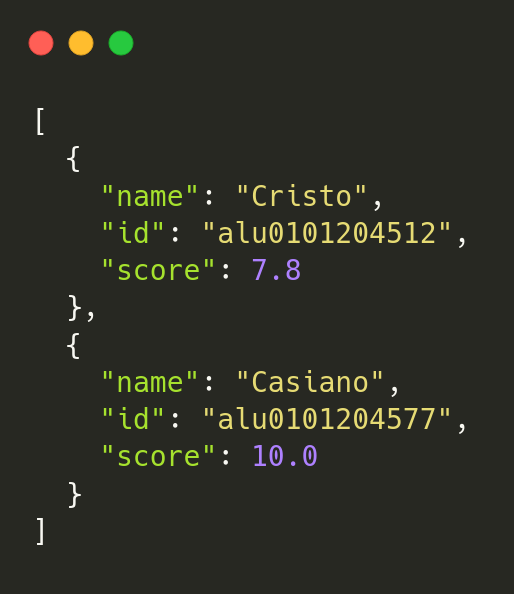
\includegraphics[width=0.5\textwidth]{images/inputJSON.png}}
    \caption{gh edu data log. Ejemplo de archivo de entrada}
    \label{fig:inputJSON}
\end{figure}

\begin{figure}[H]
    \centering
    \makebox[\textwidth][c]{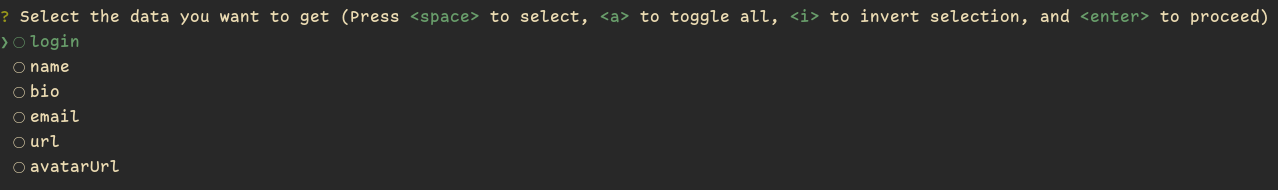
\includegraphics[width=\textwidth]{images/data-select-desiredField.png}}
    \caption{gh edu data log. Seleccionando los datos deseados}
    \label{fig:data-desiredData}
\end{figure}

\begin{figure}[H]
    \centering
    \makebox[\textwidth][c]{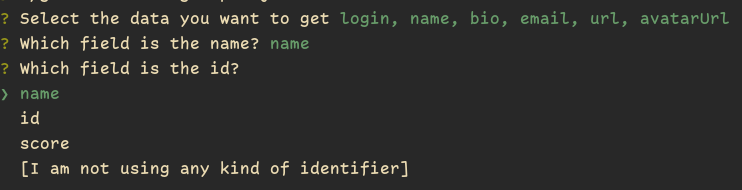
\includegraphics[width=\textwidth]{images/selectFields.png}}
    \caption{gh edu data log. Enlazando los campos del fichero de entrada con el nombre y el ID}
    \label{fig:linkFields}
\end{figure}

\begin{figure}[H]
    \centering
    \makebox[\textwidth][c]{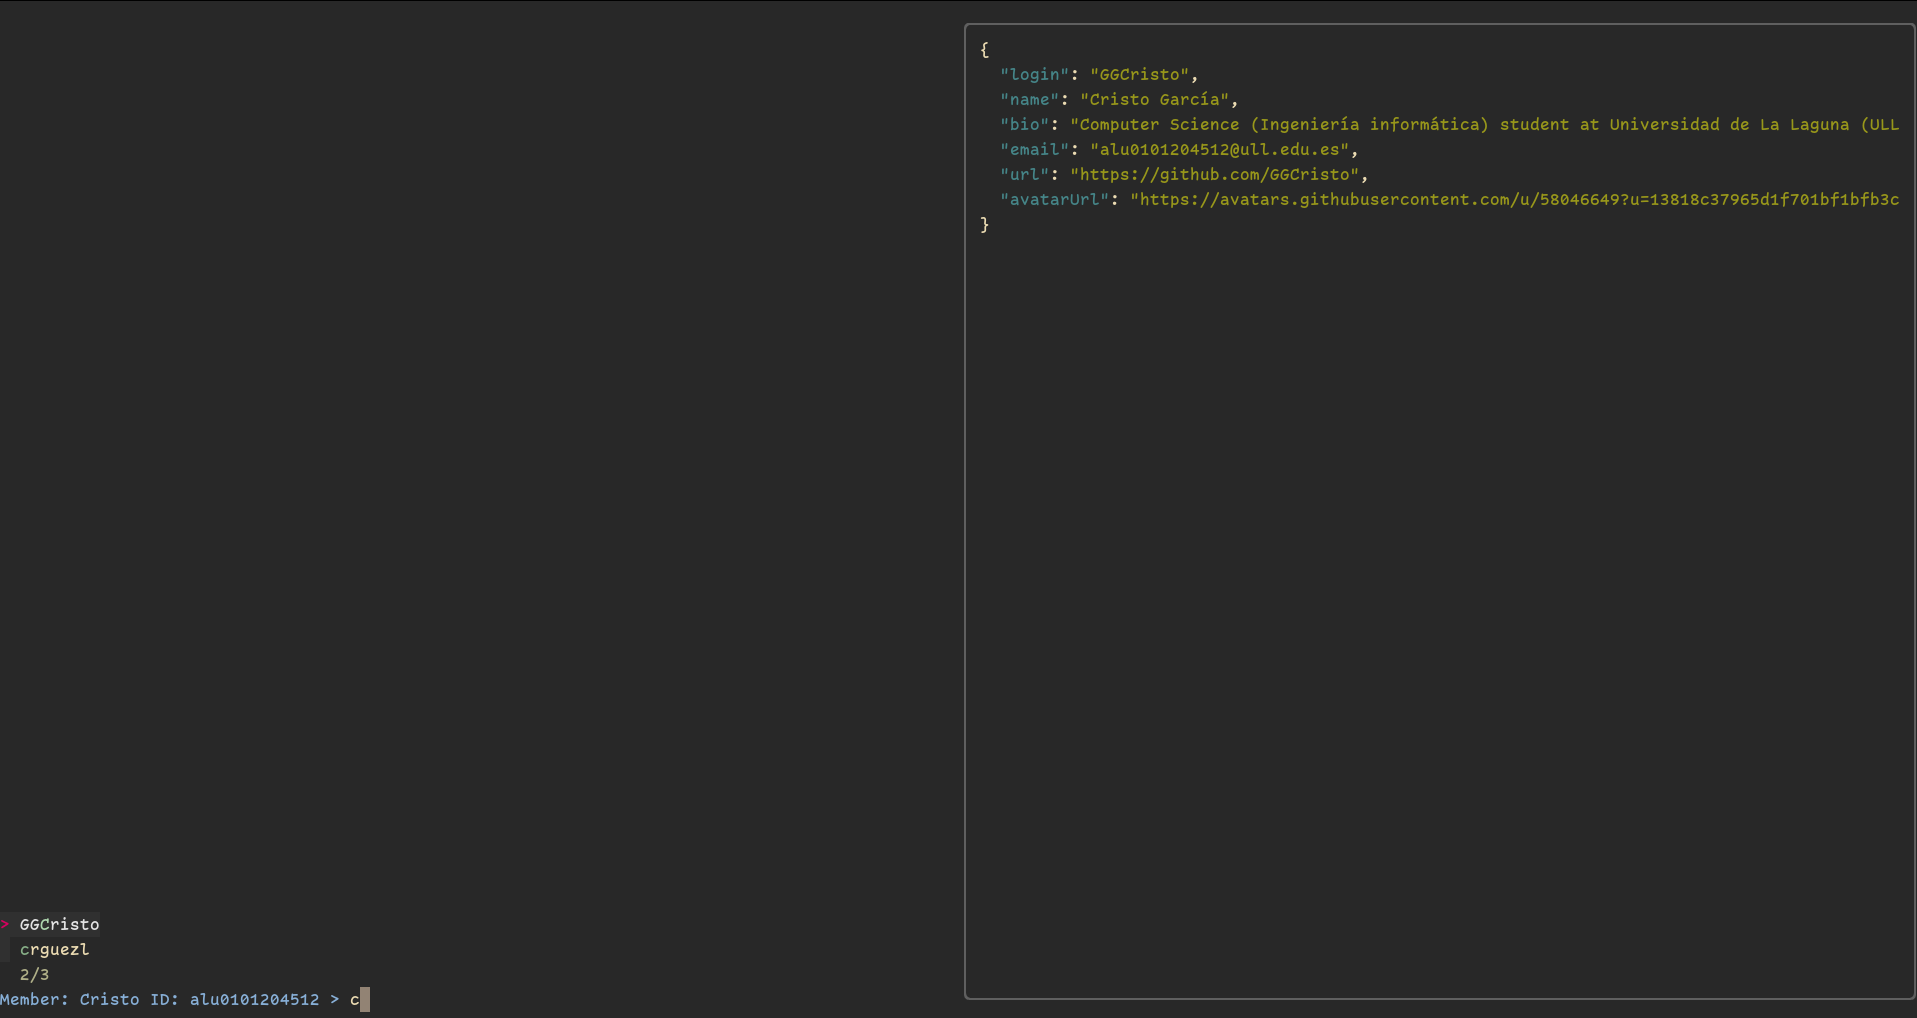
\includegraphics[width=\textwidth]{images/interface-log.png}}
    \caption{gh edu data log. Interfaz principal}
    \label{fig:interface-log}
\end{figure}

\begin{figure}[H]
    \centering
    \makebox[\textwidth][c]{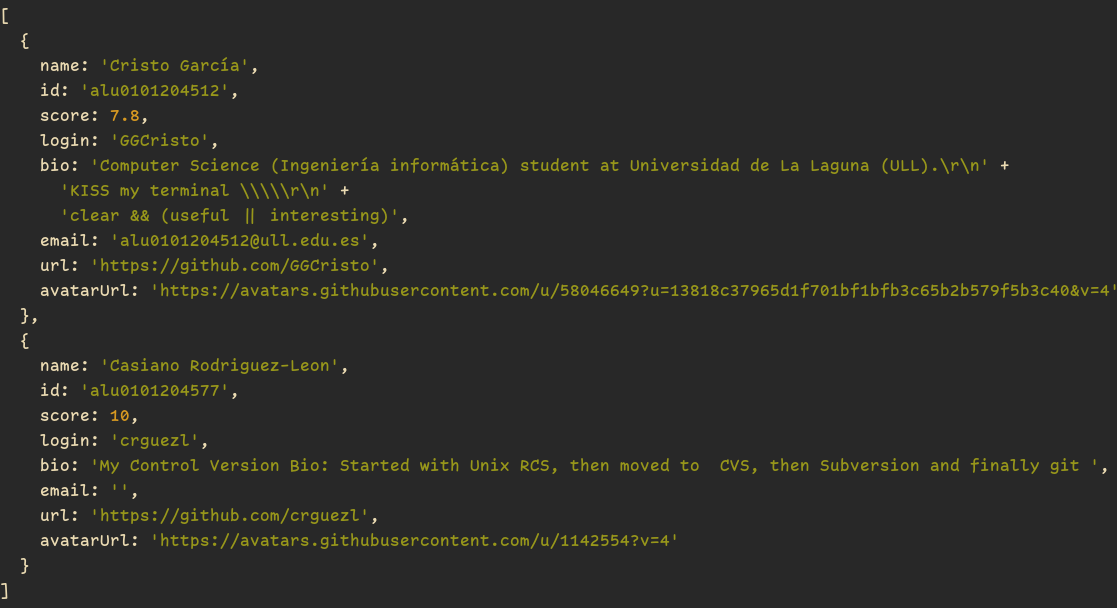
\includegraphics[width=\textwidth]{images/result-log.png}}
    \caption{gh edu data log. Resultado}
    \label{fig:result-log}
\end{figure}

Tiene los siguientes \verb|flags| para modificar su comportamiento:
\begin{figure}[H]
    \centering
    \makebox[\textwidth][c]{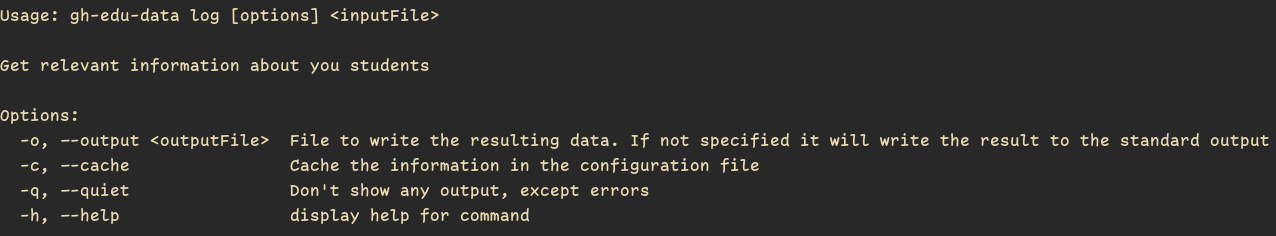
\includegraphics[width=\textwidth]{images/data-log-help.png}}
    \caption{gh edu data log. Ayuda}
    \label{fig:data-log-help}
\end{figure}

Estos \verb|flags| se comportan igual que en el resto de subcomandos, a excepción de \textbf{c, -{}-cache}, en cuyo caso, estamos indicando de que queremos guardar el resultado en una \gls{cache} en el fichero data.json. Un ejemplo del resultado se puede ver en la figura \ref{fig:data}

\subsection{El subcomando {\tt teams}}
Una de las estrategias que suelen utilizar los profesores para tener identificados a los alumnos es que en la primera práctica de la asignatura se procede a crear una asignación de GH Classroom de este modo:
\begin{enumerate}
    \item Usando una asignación de GH Classroom crear una tarea de equipo
    \item Los equipos serán individuales formados por un solo alumno
    \item Cada alumno cuando acepta la asignación crea su equipo le debe dar el nombre según las instrucciones que le haya dado el profesor
\end{enumerate}

Un ejemplo de tal instrucción del profesor sobre el nombre del equipo podría ser: 

"El nombre del equipo debe estar formado por el nombre y apellidos del alumno separado por guiones, seguido del identificador de la universidad. No use tildes ni caracteres especiales".

Por ejemplo para un. alumno dela ULL podría ser algo como \verb|cristo-garcia-gonzalez-alu0101204512|. 

El comando viene gobernado por la expresión regular con paréntesis con nombre 
especificada en la entrada \verb|teamR| del fichero de configuración:
\begin{verbatim}
➜  gh-edu-data git:(casiano) ✗ gh edu get -c | jq '.teamR'
"(?<name>.+)[-_](?<id>.+)"
➜  gh-edu-data git:(casiano) ✗ gh edu get -t
(?<name>.+)[-_](?<id>.+)
\end{verbatim}
Esta expresión regular permite decidir que \verb|name| es la primera parte \verb|cristo-garcia-gonzalez| y que \verb|id| es \verb|alu0101204512|.

\verb|teams| es un comando que tiene el mismo objetivo que \verb|log|, pero se aprovecha de esta estrategia, para que la obtención y búsqueda de dicha información sea inmediata.

El comando actúa sobre la organización por defecto. 
Supongamos fijada la organización de una cierta clase:

\begin{verbatim}
➜  gh-edu-data git:(casiano) ✗ gh edu get -o
ULL-ESIT-PL-2122
\end{verbatim}

El comando tiene las siguientes opciones:

\begin{verbatim}
➜  gh-edu-data git:(casiano) ✗ gh edu data teams -h
Usage: gh-edu-data teams [options]

Get relevant information about you students using teams

Options:
  -o, --output <outputFile>  File to write the resulting data. If not specified
                             it will write the result to the standard output
  -c, --cache                Cache the information in the configuration file
  -q, --quiet                Don't show any output, except errors
  -h, --help                 display help for command
\end{verbatim}

Entonces cuando se ejecuta:

\begin{verbatim}
➜  gh-edu-data git:(casiano) ✗ gh edu data teams
\end{verbatim}

Se conecta a la API de GH para obtener los equipos de un solo miembro he intenta obtener del nombre y propiedades de los equipos de un solo miembro la información necesaria.

Saldrá por stderr mensajes de advertencia para los equipos con mas de un miembro, como este::

\begin{verbatim}
➜  gh-edu-data git:(casiano) ✗ gh edu data teams
Warning! Teams with several members not included in the identification process: {
  "casiano-rodriguez-leon-crguezl": [
    "https://github.com/crguezl",
    "https://github.com/algorithms-ull"
  ]
}
\end{verbatim}

y por stdout saldrá algo como esto:

\begin{verbatim}
[
  {
    "url": "https://github.com/AdalDiazFarina",
    "email": "",
    "nameInGH": "Adal Díaz Fariña",
    "name": "adal-diaz-fariña",
    "id": "alu0101112251"
  },
  ... etc.
  {
    "url": "https://github.com/CorEHarD5",
    "email": "sergiodlbg@gmail.com",
    "nameInGH": "alu0100953275",
    "name": "sergio-barrera-garcia",
    "id": "alu0100953275"
  }
]
\end{verbatim}

\subsection{El subcomando {\tt team-add}}
Este subcomando fue creado como respuesta al subcomando \verb|teams| con la intención de también facilitar el trabajo a los alumnos, a la hora de crear los equipos en la organización.

Se aprovecha del campo \verb|teamR| para saber que datos pedirle al alumno. Por ejemplo, si se tiene en \verb|teamR| el siguiente valor \verb|(?<name>.*?)\.(?<id>.*?)\.(?<age>.*[^s*])|. El programa le preguntará al alumno por \verb|name|, \verb|id| y \verb|age|. Y creará un equipo en la organización especificada por \verb|defaultOrg|, con dichos datos y el alumno como miembro.

\begin{figure}[H]
    \centering
    \makebox[\textwidth][c]{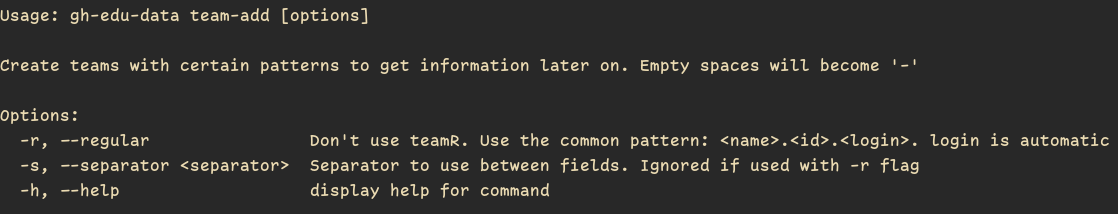
\includegraphics[width=\textwidth]{images/team-add-help.png}}
    \caption{Ayuda para subcomando team-add}
    \label{fig:team-addHelp}
\end{figure}

\begin{itemize}
    \item \textbf{-r, -{}-regular.} Ignora el campo \verb|teamR| y el flag \textbf{-s, -{}-separator}. Le pregunta al alumno por su nombre e identificador y crea un equipo con dicha información, más su identificación en GitHub. El separador es \lq.\rq. Se ha considerado que este patrón es lo suficientemente conveniente, para justificar un \verb|flag| exclusivo para él.
    \item \textbf{-s, -{}-selector.} No se ha encontrado una manera fiable de deducir el selector a partir de \verb|teamR|, por lo que el alumno tendrá que especificarlo con este \verb|flag|. Si se omite, el programa le preguntará al usuario de forma interactiva.
\end{itemize}

\section{La Extensión {\tt plagiarism}}
Es una extensión para detectar el porcentaje de similitud en las tareas de los alumnos. Se puede usar principalmente para ayudar al profesor a detectar plagio.

Genera un grafo mostrando los porcentajes y el número de líneas que son similares entre cada par de alumnos, y un informe con un enlace para ver las similitudes del código fuente.\\
Es necesario tener instalados varías dependencias:
\begin{enumerate}
    \item \textbf{MOSS (Measure Of Software Similarity)\cite{MOSS} script.} El usuario tiene que solicitar un fichero en el que viene incluido la \emph{key}/\emph{id} correspondiente. Los pasos del proceso están en su \href{https://theory.stanford.edu/~aiken/moss/}{página web}.
    \item \textbf{Perl.} Para poder ejecutar el script de \verb|MOSS|.
    \item \textbf{mossum\cite{mossum}.} Para generar el grafo con los datos de \verb|MOSS|.
\end{enumerate}
\verb|fzf| es opcional
\begin{figure}[H]
    \centering
    \makebox[\textwidth][c]{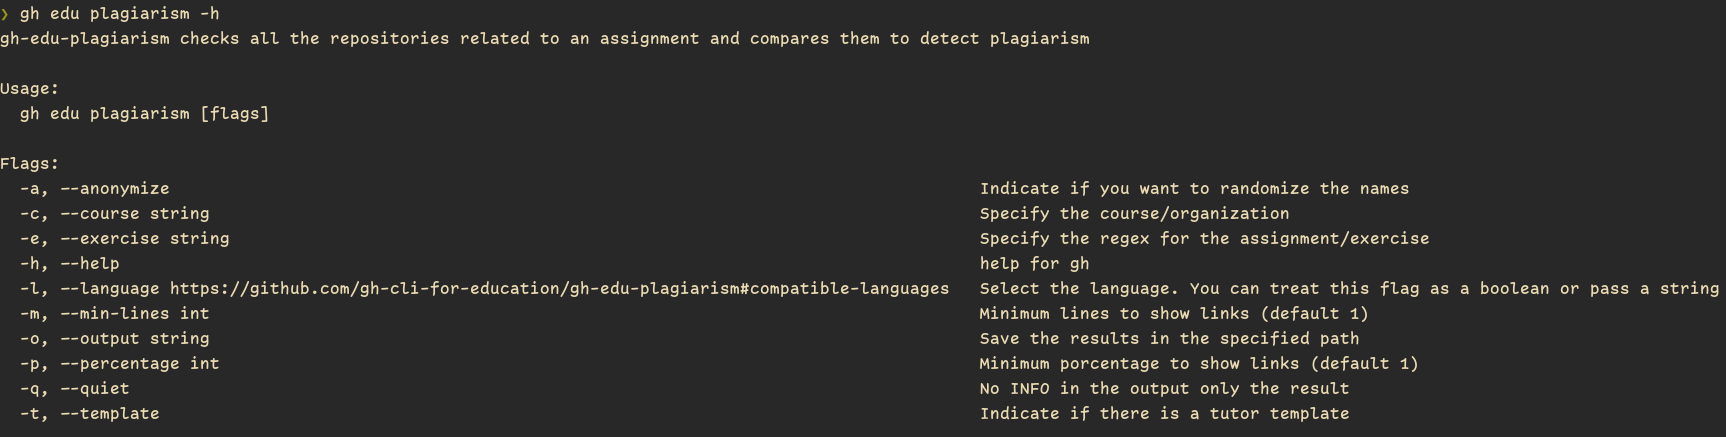
\includegraphics[width=\textwidth]{images/plagiarism-help.png}}
    \caption{Ayuda de gh edu plagiarism}
    \label{fig:plagiarismHelp}
\end{figure}

\begin{itemize}
    \item \textbf{-a, -{}-anonymize}, muestra el grafo con nombres falsos aleatorios. Se podría usar en caso de que el profesor quiera mostrar el grafo a la clase.\\
    \emph{Nota: Este comando solo se aplica al grafo, el informe se queda intacto, ya que está destinado a ser consumido únicamente por el profesor}
    \item \textbf{-c, -{}-course <course>}. La organización se puede indicar con este flag, y toma prioridad con respecto al archivo de configuración.
    \item \textbf{-e, -{}-exercise <exercise>}. La expresión regular para la tarea se puede indicar con este flag, y toma prioridad con respecto al archivo de configuración.
    \item \textbf{-l, -{}-language <language>}. Indica el lenguaje de programación utilizado.\\
    A pesar de que esta sea un campo obligatorio para que funcione el programa, si se omite se pedirá más tarde de forma interactiva con \verb|fzf|
    
    Se aceptan los mismos lenguajes que \verb|MOSS| acepta, los cuales son: c, cc (C++), java, ml (Meta Language), pascal, ada, lisp, scheme, haskell, fortran, ascii, vhdl, perl, matlab, python, mips, prolog, spice, vb (Visual Basic), csharp (C\#), modula2, a8086 (8086 assembly), javascript, plsql (PL/SQL), verilog.
    \item \textbf{-m, --min-lines <lines> (Por defecto: 1)}. Indica cuál es el número mínimo de líneas que deben ser similares para que el estudiante salga en el grafo.
    \item \textbf{-o, --output <path>}. Indica donde se quiere guardar el resultado. El informe y el grafo se guardan en el directorio temporal del sistema hasta la siguiente ejecución, utilizando este flag se puede indicar donde guardar los resultados de forma persistente.
    \item \textbf{-p, -{}-percentage <percentage>(Por defecto: 1)}. Indica cuál es el porcentaje mínimo de similitud entre los pares para mostrar en el grafo.
    \item \textbf{-q, -{}-quiet}. No se muestra ninguna información, aparte del informe final. Útil para redirigir el informe a otro fichero.
\end{itemize}